%%%%%%%%%%%%%%%%%%%%%%%%%%%%%%%%%%%%%%%%%%%%%%%%%%%%%%%%%%%%
%%% ELIFE ARTICLE TEMPLATE
%%%%%%%%%%%%%%%%%%%%%%%%%%%%%%%%%%%%%%%%%%%%%%%%%%%%%%%%%%%%
%%% PREAMBLE 
\documentclass[9pt,lineno]{elife}

\usepackage[export]{adjustbox}
\usepackage{lscape}
\usepackage{afterpage}
\usepackage{hyperref}
\hypersetup{
    colorlinks=true,
    linkcolor=blue,
    filecolor=magenta,      
    urlcolor=cyan,
}

\newcommand{\sgcomment}[1]{\textcolor{blue}{SG: #1}}
\newcommand{\luke}[1]{\textcolor{blue}{Luke: #1}}
\newcommand{\todo}[1]{\textcolor{blue}{*#1*}}
\newcommand{\alex}[1]{\textcolor{red}{Alex: #1}}
%%%%%%%%%%%%%%%%%%%%%%%%%%%%%%%%%%%%%%%%%%%%%%%%%%%%%%%%%%%%
%%% ARTICLE SETUP
%%%%%%%%%%%%%%%%%%%%%%%%%%%%%%%%%%%%%%%%%%%%%%%%%%%%%%%%%%%%
\title{Legacy Data Confounds Modern Genomics Studies}

\author[1,2]{Luke Anderson-Trocm\'e}
\author[1,2]{Mathieu Bourgey}
\author[1,2]{Rick Farouni}
\author[3]{Fumihiko Matsuda (and coauthors)}
\author[1,2]{Simon Gravel}

\affil[1]{Department of Human Genetics, McGill University, Montreal, QC H3A 0G1, Canada}
\affil[2]{McGill University and Genome Quebec Innovation Centre, Montreal, QC H3A 0G1, Canada}
\affil[3]{Center for Genomic Medicine, Graduate School of Medicine, Kyoto University, Kyoto 606-8501, Japan}
\corr{simon.gravel@mcgill.ca}{SG}

%%%%%%%%%%%%%%%%%%%%%%%%%%%%%%%%%%%%%%%%%%%%%%%%%%%%%%%%%%%%
%%% ARTICLE START
%%%%%%%%%%%%%%%%%%%%%%%%%%%%%%%%%%%%%%%%%%%%%%%%%%%%%%%%%%%%

\begin{document}

\maketitle
\begin{abstract}
In investigating an unusual population genetics signal we identified a strong and previously unreported batch effect in the 1000 Genomes Project data.
We also found that this batch effect led to spurious results in a number of recent publications. 
We identified spurious mutations by correlating mutations with data quality metrics.
We then turned our attention to the rest of the 1000 Genomes populations and saw that there were similar batch effects in many of these populations.
Some of these variants are being imputed onto genotype data and reach genome wide significance in recent publications.
\end{abstract}

\section{Introduction}
		
\subsection{Reference Cohorts}			

The last 5 years have seen a drastic increase in the amount and quality of human genome sequence data. 
Hapmap \cite{HapMap2005}, the 1000 Genomes Project \cite{1000GenomesProjectConsortium2010,The1000GenomesProjectConsortium2012}, and the Simons Diversity project \cite{Mallick2016}, for example, have made thousands of genomes publicly available for population and medical genetic analyses. 
Many more genomes are available indirectly through servers providing imputation services \cite{ProfJonathanMarchiniProfGoncaloAbecasisProfRichardDurbin2014} or variant frequency estimation \cite{Lek2016}. 

Many of these large datasets have been assembled over several years using a variety of sequencing platforms. 
The first sequenced genomes in the 1000 Genomes project (1kGP), for example, were sequenced 10 years ago.
During this period, sequencing platforms were still being rapidly developed.
This lead to heterogeneous sample preparations for many of the samples included in the dataset.
Because of the extraordinary value of freely available data, this early data from the 1kGP is still widely used as a reference panel for imputation, allele frequency estimations and a wide range of applications. 

Although, it is clear that the quality and accuracy of the 1kGP data has increased over the past decade. 
This data is far from perfect, the publication from the second phase of the 1kGP describe technological and analytical improvements over its previous phases.
This raises the question of whether and how such legacy data should be included in contemporary analyses alongside more recent cohorts. 
Here we point out how large and previously unreported batch effects in the early phases of the 1kGP that still lead to incorrect genetic conclusions through population genetic analyses and indirect use through prominent imputation servers.  

\subsection{Motivations}

Genome wide mutational signatures have been used as a diagnostic tool for cancers \cite{Pleasance2010,Shiraishi2015a}.
Certain mutagens in tobacco smoke, for example, have been shown to preferentially bind to certain genomic motifs leading to an excess of G to T transversions \cite{Pleasance2010}.
This means that the genomic context of a mutation can be used to gain insight into the cause of this mutation \cite{Pleasance2010}.
While certain mutagens have very distinct mutational signatures, others are more subtle and difficult to identify because they tend to occur less frequently and with less genomic specificity [\cite{}].
Large cohorts have recently become available to increase statistical power to resolve some of these fine scale mutational signatures.

Fine scale mutational signatures are observable on evolutionary scales by comparing the rates of mutations between populations.
In 2015, Harris reported 50\% more TCC ${\rightarrow}$ TTC mutations in European populations compared to African populations; this was replicated in a different cohort in 2017 \cite{Harris2015a}.
A more in depth analysis of these subtle mutational signatures was recently released in preprint by Aikens, Johnson and Voight. \cite{}
In their study they expanded the investigations of mutational signals in the 1kGP by investigations to broader sequence contexts.

This strong population enrichment of a mutational signature suggests important genetic or environmental differences in the history of each population \cite{Harris2015a}. 
Harris and Pritchard further identified distinct mutational spectra across a range of populations \cite{Harris2017a}. 
In particular, they identified a heterogeneous mutational signature within 1000 Genomes Japanese individuals.
In addition, multiple 7-mer mutational signatures were also identified by Aikens et. al in the same populations. \cite{}
Such an axis of variation is intriguing because differences in mutational signatures accumulate over many generations.
A systematic difference among the Japanese population would suggest sustained environmental or genetic differences across sub-populations within Japan with little to no gene flow.
We therefore decided to follow up on this observation, by using a newly sequenced dataset \sgcomment{description of cohort.}

While we were unable to reproduce the heterogeneity among the Japanese population, we could trace back the source of the discrepancy between the two datasets and identified a strong and previously unreported batch effect in the 1kGP data.
We also found that this batch effect led to spurious results in a number of recent publications. 

This study is the result of an investigation in the quality of the 1kGP dataset. 
To begin, we will discuss how we discovered these previously unreported batch effects in the 1kGP. 
Next, we explore more broadly how low quality data remain embedded in other populations of the 1kGP. 
Finally, we will discuss the ways in which it contaminated a number of recent studies.
Fortunately, the main conclusions of most of these studies remain supported by other data.
Yet this begs the question: When should we retire legacy data?

\begin{figure}
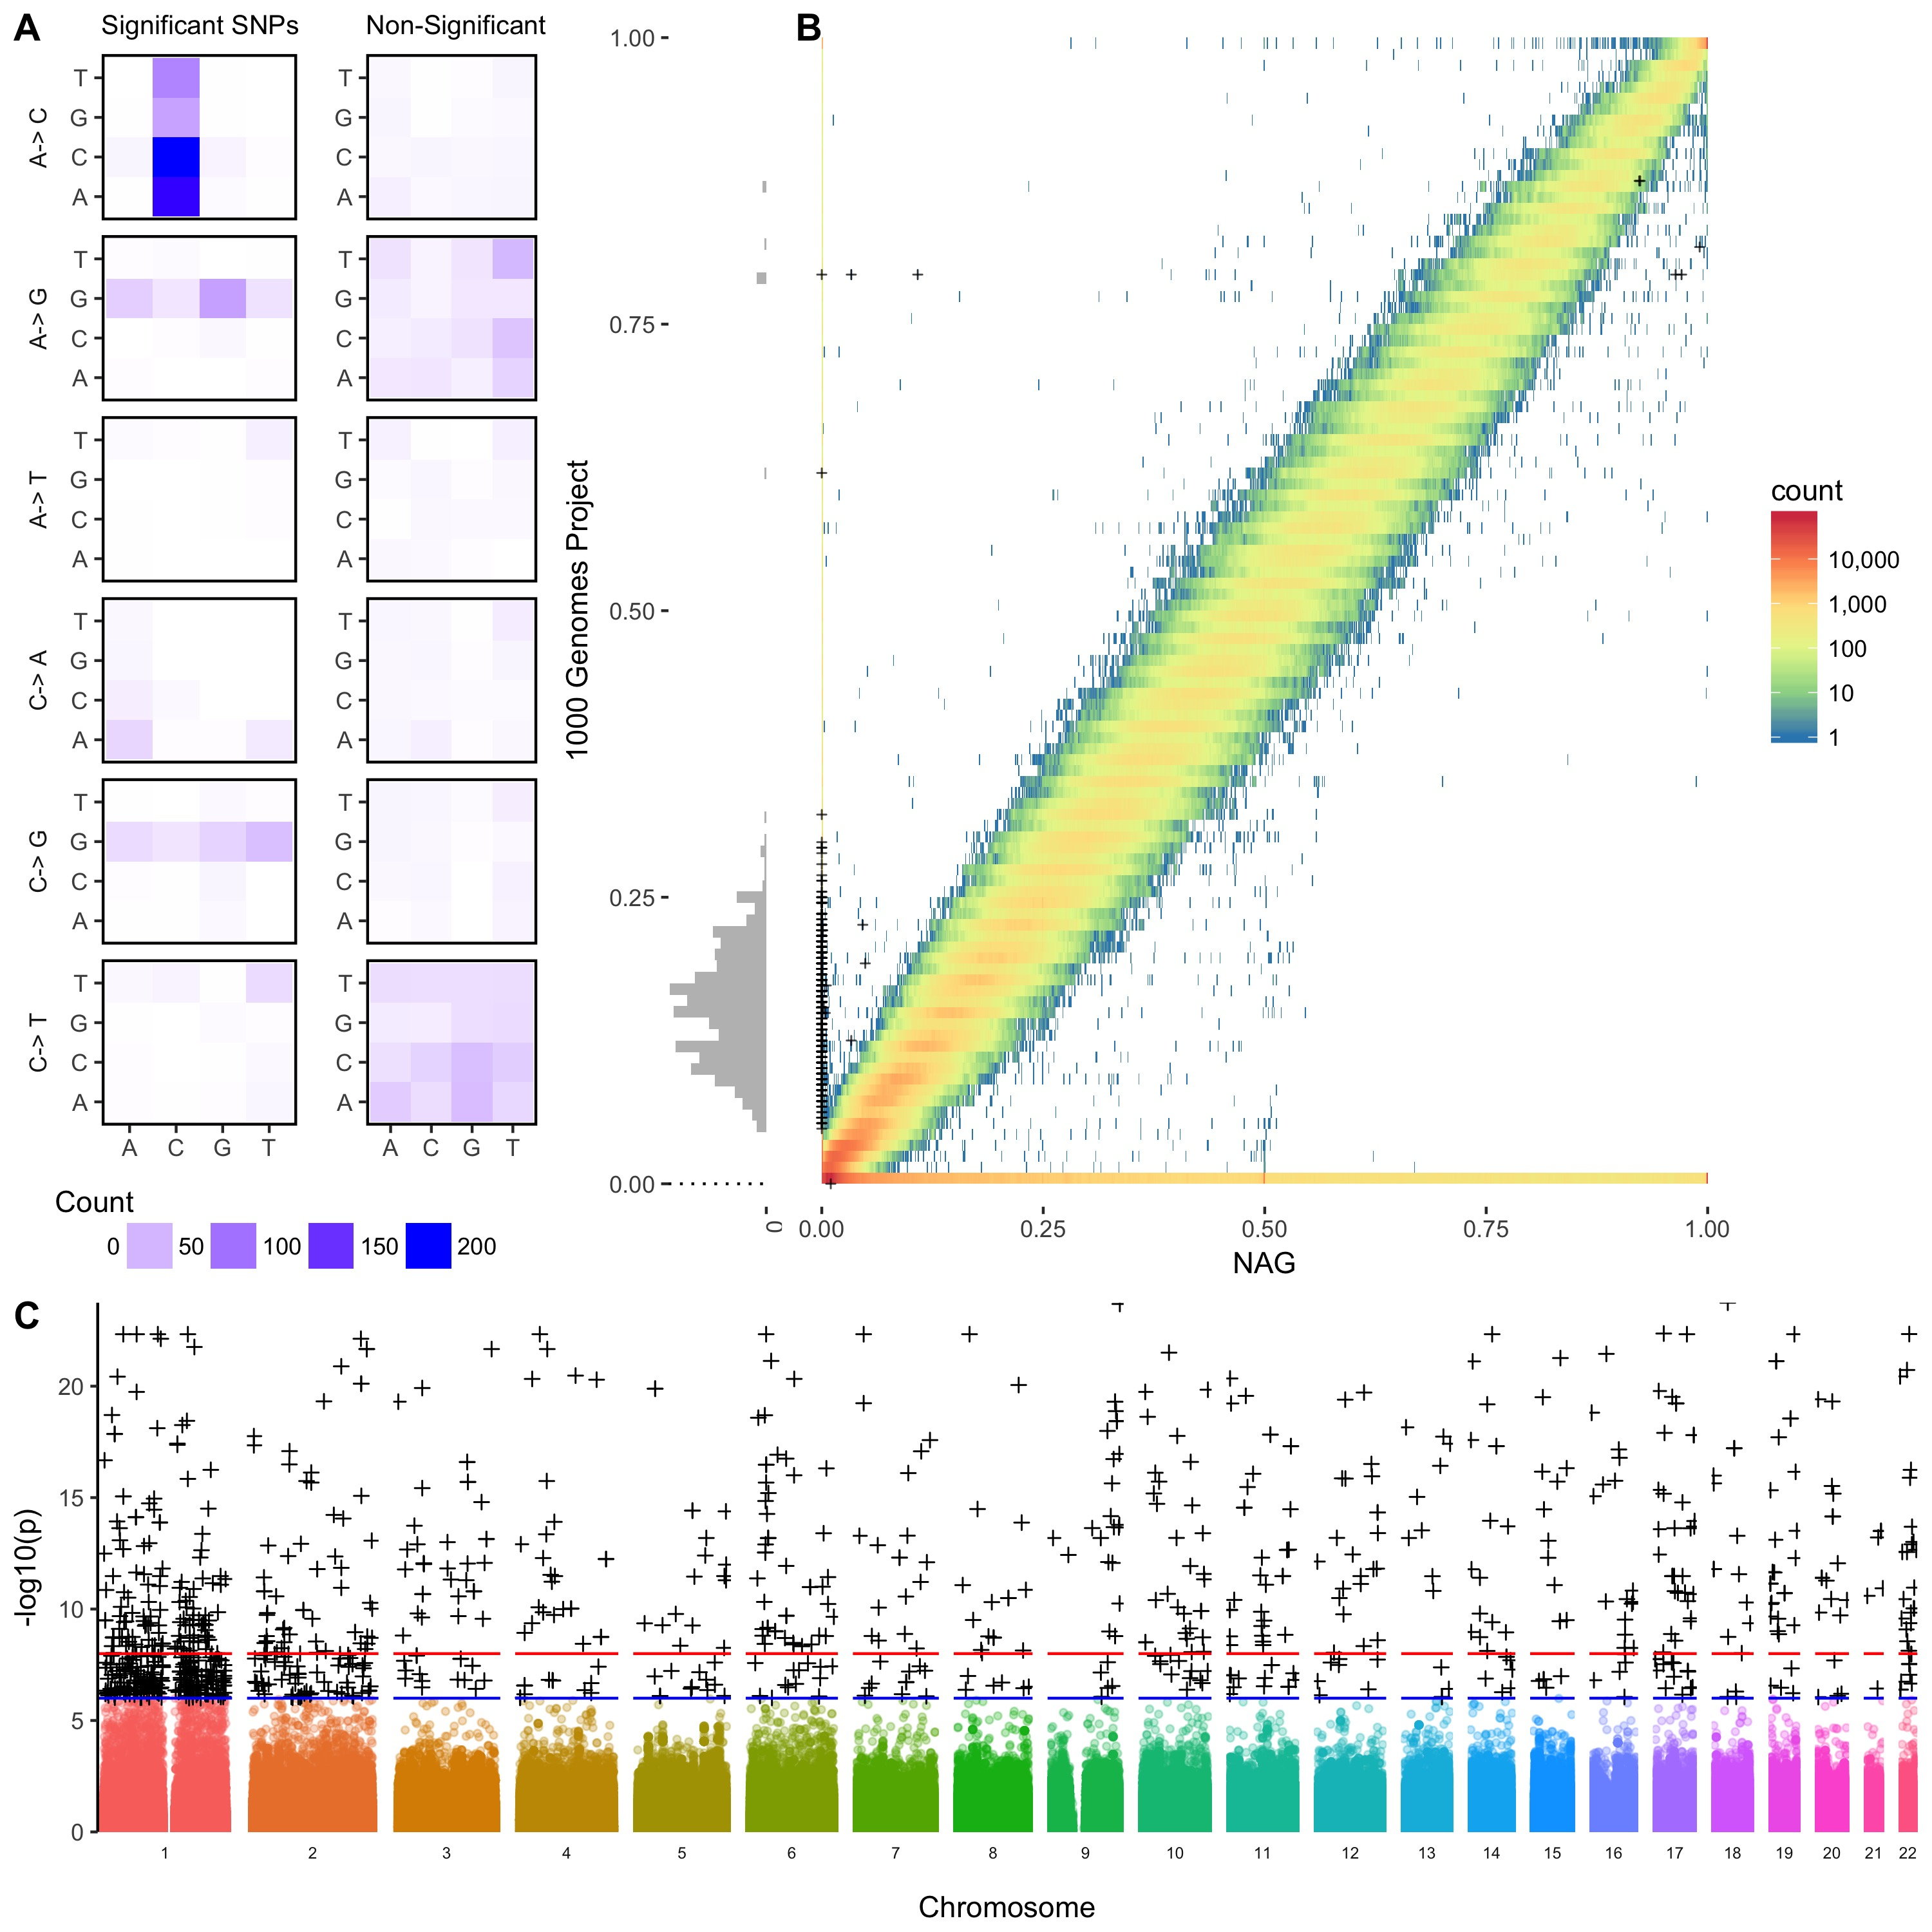
\includegraphics[width=\hsize,keepaspectratio]{Figure1.jpg}
\caption{
\textbf{A} 
Mutation spectrum of the 1034 variants that reached a genome wide significance with a p value less than $p < 10^{-6}$  in a GWAS of sequencing quality. 
There majority of the variants with significant associations to quality have the *AC${\rightarrow}$*CC mutational pattern. There is also an slight enrichment in GA*${\rightarrow}$GG* and GC*${\rightarrow}$GG* mutations. These three enrichments can be summarized as G**${\rightarrow}$GG*. (note: the reverse complement of *AC${\rightarrow}$*CC is GT*${\rightarrow}$GG*)
\textbf{B} 
Joint frequency spectrum plot of the Japanese from the 1kGP and a more recent Nagahama dataset.
Crosses ( + ) are variants that reached genome wide significance in a GWAS of sequencing quality. 
The histogram on the left of the plot is the distribution of significant variants. 
The dotted line is at 5\% allele frequency. 
\textbf{C} 
Genome wide association of the average quality of mapped bases for the 104 Japanese individuals included in the 1kGP. This GWAS identified $587\ \  p < 10^{-8}$ and $1034\ \ p < 10^{-6}$ SNPs that were associated to the average quality of SNPs mapped for an individual
The same analysis was performed independently for each of the populations in the 1kGP. }
 \label{SFS}
\end{figure}

			\section{Results}
	\subsection{A peculiar mutational signature in Japan}			
	
Harris and Pritchard reported an excess of a 3-mer *AC${\rightarrow}$*CC mutational pattern in a portion of the Japanese individuals in the 1kGP.\cite{Harris2015a}
While trying to follow up on this observations in a larger and more recent Japanese cohort, we did not find this particular signature.
However, when comparing the allele frequencies between the Japanese individuals from the 1kGP and this larger dataset, we observed an unusually large number of private single nucleotide polymorphisms (SNPs), only found in one of the two groups.
This is unexpected given the similarity of the two populations, and suggests a technical artifact rather than a population structure effect. 
Moreover, these mismatches were maintained after filtering for low-quality regions of the human genome and standard metrics such as Hardy-Weinberg equilibrium.

When mismatch sites were removed from the 1kGP data, the  *AC${\rightarrow}$*CC signal disappears \ref{SFS}.
Regressions against different individual-level quality metrics provided by the 1kGP revealed that mean quality per mapped base pair per individual was an excellent correlate with prevalence of the  *AC${\rightarrow}$*CC mutational signature in 1kGP. 
Individuals with low-quality data showing elevated rates of the signature (see Supplementary Figure \ref{PC1_Correlation}).
Thus sequences with low mappability harbour mutations that reproduce poorly across studies and exhibit a particular mutational signature. 

To identify SNPs that are likely to reproduce poorly across cohorts (without having access to a second cohort), we performed a genome-wide association study (GWAS) in the JPT for SNPs that correlate strongly with low quality \ref{SFS}.
\luke{NEW:} 
Whereas the majority of GWAS use linear regression predicting a phenotype based on genotype, our method does the inverse.
We are looking for loci where the genotypes are predictable based on the data quality scores.
We were able to identify 587 SNPs with $p < 10^{-8}$ and 1034 SNPs with $ p < 10^{-6}$.
While identifying putative low-quality SNPs to exclude, using a higher $p$-value threshold increases the stringency of the filtering (i.e., the traditional genome-wide significance threshold might not be a good guide for filtering).  
 %This GWAS included 104 Japanese individuals, 74 of which were sequenced in using the Genome Analyzer II while the rest were sequenced using the HiSeq 2000 of the 1kGP.
The variants that are associated to the quality of mapped bases have an enrichment in *AC${\rightarrow}$*CC mutations. 

The signal is enriched in GWAS SNPs, but residual signal remains presumably because many rare alleles found in individuals with low-quality data remain unidentifiable using association techniques.
For this reason, the heterogeneously distributed signal persisted in the 1kGP Japanese even after filtering the variants that were significantly associated to quality.
The *AC${\rightarrow}$*CC mutational signal is limited to individuals with low quality sequencing data.
Therefore, the removal of individuals with average qualities below 30 successfully removes the signal.
While the GWAS approach can identify some of the low hanging bad apples, there are likely more of these false positives nested inside these legacy cohorts.

%Many of the populations in the 1kGP do not have higher quality counterparts which means that identifying questionably low quality data must be done ad hoc.

	\subsection{Sequencing quality over time}
The results of the GWAS performed on the Japanese from the 1kGP lead us to consider whether any other populations in the 1kGP also had similar issues with data quality.
The average quality of sequencing data of individuals over time shows that the sequencing done in the early phases of the 1kGP was more variable and overall tended to include lower quality sequencing data \ref{MapQual}.
This variability could be as a result of fluctuating sequence platform protocols or variation between sequencing centres.
There were a number of protocols used to prepare the samples for sequencing, as well as a number of sequencing technologies used over the course of the data production.
By 2011, older sequencing technologies are phased out, and method development solidify, which coincides with the sequencing quality levelling off.

\begin{figure}
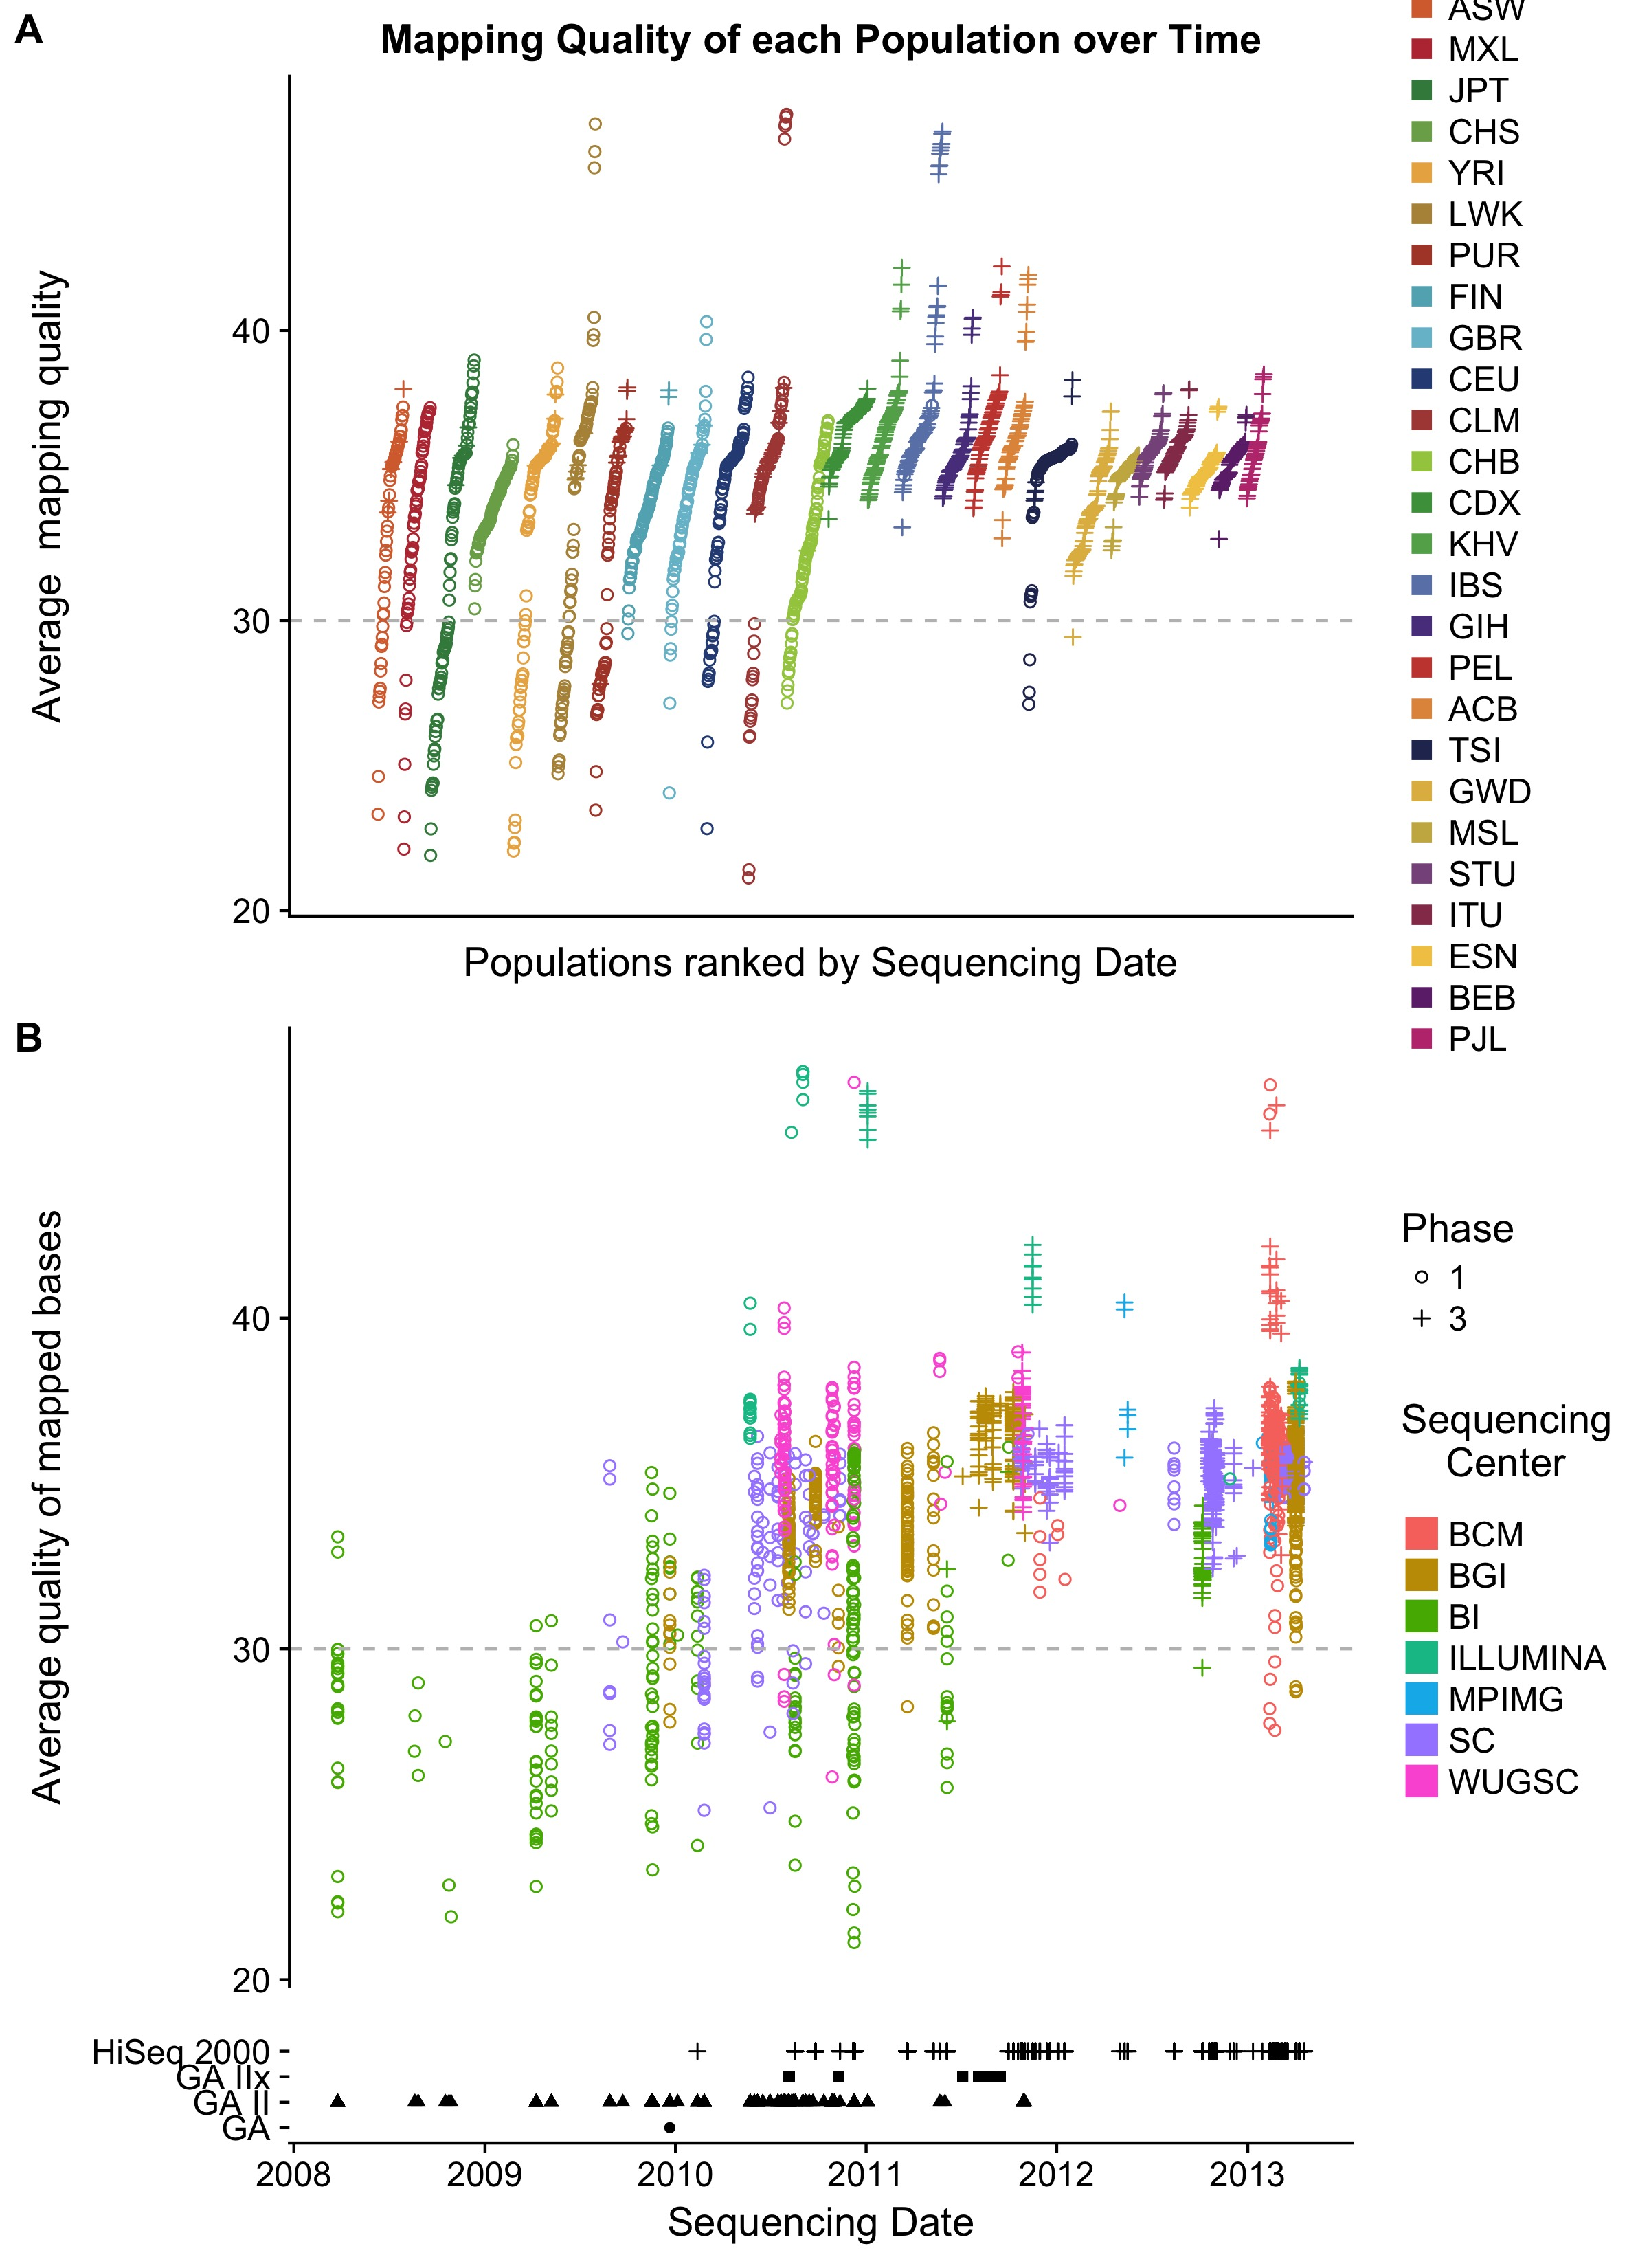
\includegraphics[width=\hsize,keepaspectratio]{MapQualOverTime.jpg}

\caption{\textbf{A} The average mapping quality of each individual per population included in the 1000 Genomes sequencing project. The x-axis is ranked by populations with the lease to the most variance, followed by average mapping quality per individual. \textbf{B} Same data as in \textbf{A} except the x-axis is sorted by sequencing date. The colours indicate the sequencing centers that produced the data for each individual.}
\label{MapQual}
\end{figure}

	\subsection{Overlap of significant SNPs}
We applied the same GWAS approach on the other 1kGP populations as it appears to capture a large portion of problematic sites. 
We found that 24 of the 26 populations in the 1kGP had SNPs significantly associated to the average quality of mapped bases per individual.
Comparing the results of each independent GWAS, we were able to identify over 3517 variants that were independently associated to low quality in at least two populations  \ref{OverLap}. 

\begin{figure*}
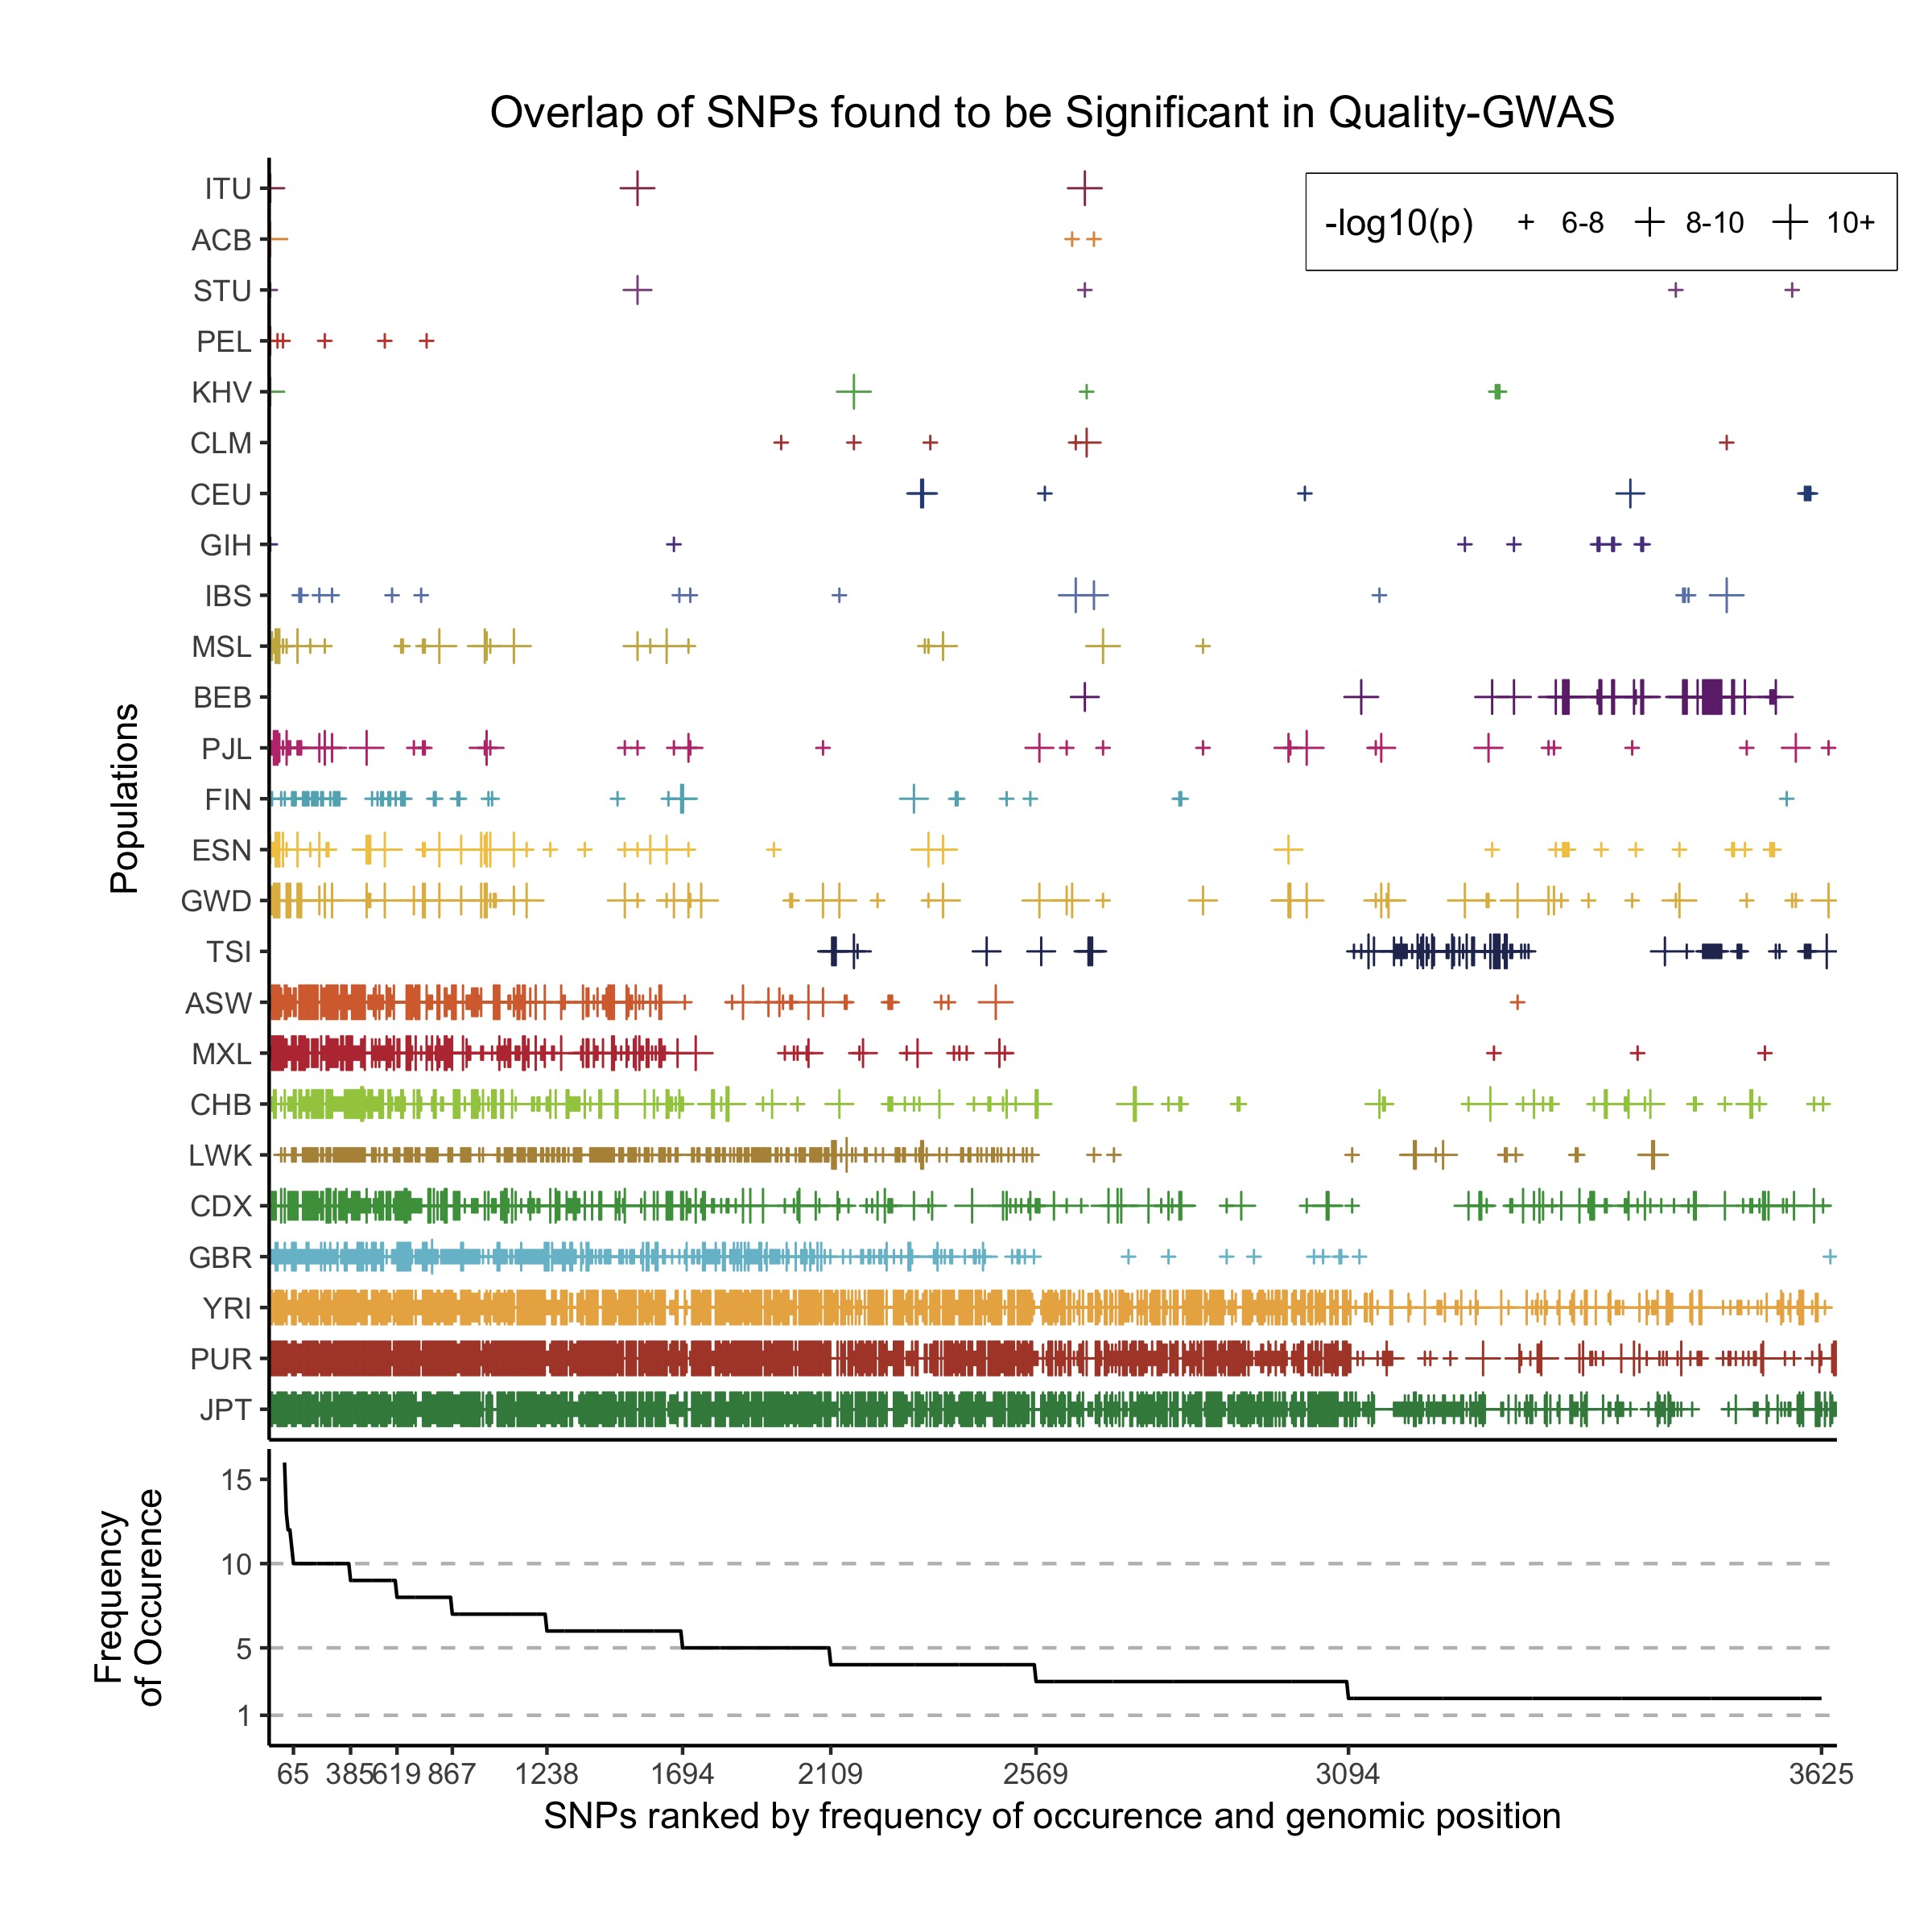
\includegraphics[width=\hsize,keepaspectratio]{SNPOverlap6.jpg}

\caption{Overlap of SNPs identified independently to be associated with quality. 
The size of the crosses ( + ) are proportional to the -log10(p) value of that SNP.
The x axis is ranked by the frequency of occurrence of a SNP, then by genomic position.
The line plot underneath shows the number of populations for which a variant has reached significance.
The populations that tend to have the most low-quality individuals also tend to have the most variants associated to quality. 
The same variants identified as being low quality independently in each population are found in other populations. }
  \label{OverLap}
\end{figure*}

\subsection{Combined Test}
To improve on the power of our test, we performed a test by combining the deviations from the null model for each SNP for each population.
Each population will have it's own deviation from the null for each position in the genome.
We computed the combined p value for each position by taking the sum of the deviations from each population and adjusting the degrees of freedom for the chi-squared test according to the number of populations with a segregating variant.
This resulted in an increase in the number of SNPs reaching genome wide significance to 3664. \ref{Manhattan}

\begin{figure*}
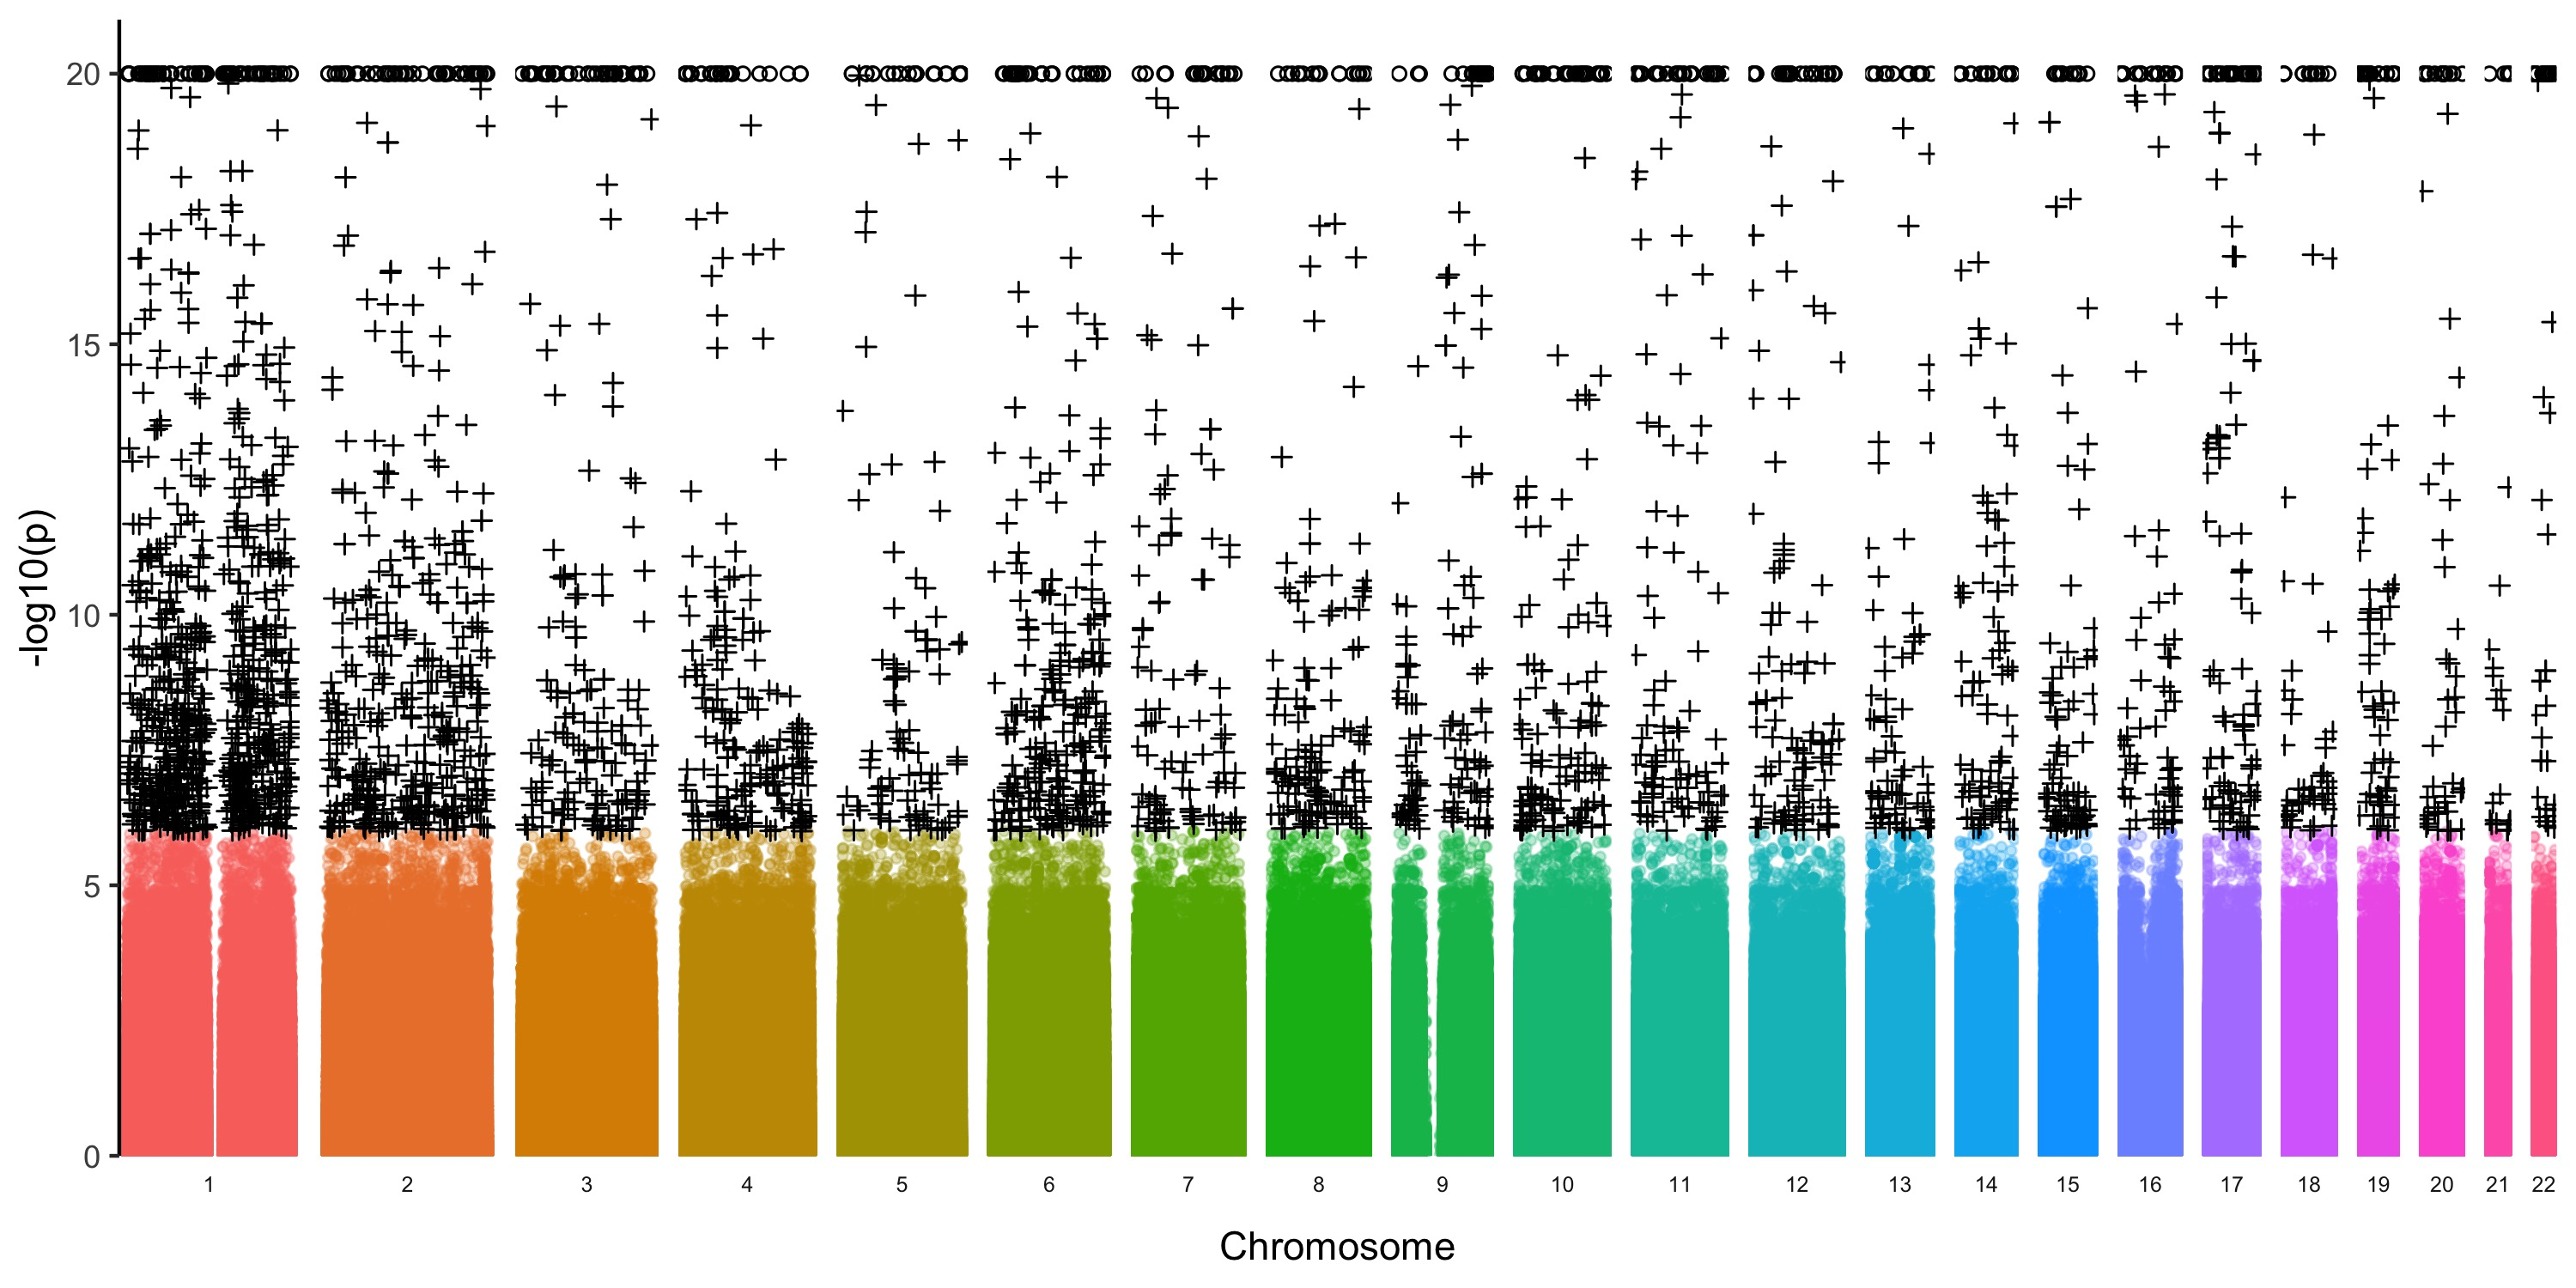
\includegraphics[width=\hsize,keepaspectratio]{ManhattanPlot.jpg}

\caption{Manhattan plot of the -log10 p values for the combined test using the deviations from each population of the 1kGP. 
There are 2007 and 3664 variants that reach p values greater than $ p < 10^{-8}$ and $ p < 10^{-6}$ respectively.
Crosses ( + ) represent SNPs that reach a genome wide significance greater than $ p < 10^{-6}$, the circles ( o ) are SNPs that reached values greater than 20, for clarity we implemented hard ceiling at 20.}
  \label{Manhattan}
\end{figure*}

	\subsection{Imputation}
The state of the art imputations servers use a combination of many databases including many that are not freely available.
For this reason, the details of the methods used to impute genomic data are not publicly available either.
In order to investigate the proportion of variants that we've identified as being associated to quality that are being imputed, we submitted genotype data from the 1kGP and imputed it using the Michigan Imputation Server.
We found that all of the SNPs we identified as being associated with quality were imputed.
This suggests that the imputation reference panel includes individuals with low sequence quality, as well as the variants that have been shown to be associated to quality. 

	\subsection{Found to be included in other GWAS }
Once we identified SNPs that were clearly associated with low quality, we searched the literature for any GWAS that might have called these erroneous variants as being significantly correlated with some biological trait. 
Using the NHGRI-EBI Catalog of published genome-wide association studies we queried the rsIDs of the SNPs we identified as being low quality and found two recent publications that had found at least one of the variants to have reached genome wide significance in their study.

One of these studies genotyped individuals and imputed the data using the HapMapII as a reference  database for imputation. 
The other study used the 1kGP sequence data directly.
Both papers used strict quality thresholds, including population genetic statistical tests such as the Hardy-Weinberg equilibrium test, deviations in expected allele frequency and sequencing data quality thresholds. 
They also removed rare alleles and alleles with high degrees of missingness. 
Despite using the state of the art quality controls, these erroneous variants managed not only to be imputed onto real genotype data, but they also reached genome wide significance for biological traits.



\begin{center}
 \begin{tabular}{l l l r r} 
 \hline
Author & Year & Journal & RSID & PMID \\ [0.5ex] 
 \hline
Ebejer JL	& 2013	 & Twin Res Hum Genet & 	rs6057648&23527680\\ 
 
Mandage R &	2017	 & PLoS One	 & rs200655768, rs184202621,&28654678\\
& & & rs201255786, rs201761909&\\
 \hline
 \end{tabular}
\end{center}

			\section{Discussion}
%\subsection{Why do we care?}
The variants identified in this study are likely to be technical artifacts from legacy technology.
If these sequencing platforms are no longer being used then it it likely that these artifacts are no longer being actively introduced in recent sequence data.
However, because the 1kGP data is widely used as a reference database, these variants are being imputed onto new genotype data.
We have shown that these variants have been significantly associated using traditional GWAS methods.
However this is not the only method that would be affected by these false positives. 
Polygenic risk scores, meta analyses and other methods that combine the scores of multiple variants might also include some of these variants in their analyses.
The inclusion of these variants could also affect population genetics analyses that compare and contrast populations based on allele frequencies.

%\subsection{Recommendations}
The most conservative approach would be to remove all individuals that don't meet the quality threshold as well as all the variants associated to low quality.
In this case, we used a cut off of an average quality of mapped bases over 30. It is the minimum requirements for \todo{GATK variant calling} for them to have a minimum quality of 30.

%\subsection{Power limits and Quality Controls}
If these variants are truly spurious, why were they not identified by the Hardy-Weinberg test of heterozygosity?
\todo{how many hetd do you need to detect HWE significance?}
We were able to identify many variants with frequencies below \todo{the power threshold for HWE}.

%\subsection{Technical Source of Error}
%B tail trimming  (Minoche et al. Genome Biology 2011)
%issues with PCR?
%repetitive regions, GC bias...

\subsection{Twins Research Human Genetics}
Genotype + Imputation + GWAS

\subsection{PLos One}
Using 1kGP data directly, estimating count of EBV

			\section{Conclusion}
Our method identifies spurious mutations by correlating mutations with data quality metrics. 
We propose including our quality control methods to identify possible false positives in sequencing data. 
We have focused on the 1000 Genomes Project dataset as its quality metrics were freely available, however the issues of quality control are not limited to this one consortium. 
This study only used one dataset and one quality metric, but using this same approach can be used to identify more false positives in many more datasets. 

As more large scale genotyping efforts are being imputed on the same legacy datasets, we must scrutinize the quality of the reference databases to avoid the propagation of false positives. 
These results bring forth many questions regarding the reliability of legacy datasets. 
Moreover, since there are so many broad applications of imputation, it frames the question for reference data turnover. 

Many types of DNA sequencing machines have been available on the market over the past decade.
Different types of sequencing technologies can have different technical limitations in quality control.
This makes combining data an issue especially when multiple sequencing technologies are involved in the data production.
Many of the legacy datasets produced using dated sequencing technologies have been known to contain a higher rate of false positives than their more recent counterparts.
The errors in one dataset do not disappear when they are combined with another higher quality one.
The technical biases caused by legacy sequencing technology is becoming increasingly relevant as newer technologies produce data with lower error rates, and more stringent quality controls.




\section{Methods}
\subsection{Metadata}
The metadata used in this analysis was compiled from each of the index files from the 1000 Genomes file system. 
Average quality of mapped bases per sample was obtained from the BAS files associated with each alignment file. 
Each BAS file has metadata regarding each sequencing event for each sample. 
If a sample was sequenced more than once, we took the average of the each quality score from each sequencing instance. 
The submission dates and sequencing centres for each sample in the analysis was available in the sequence index files.  
This file also has multiple entries per sample, however, we were unable to match the individual sequencing runs between the bas files and the index file, which lead us to take the average of the quality scores and only kept the earliest sequencing date per sample. 
The dates of the sequencing are only used to plot Figure.

\subsection{Data Availability}

Index of BAS files \href{http://ftp.1000genomes.ebi.ac.uk/vol1/ftp/data_collections/1000_genomes_project/1000genomes.low_coverage.GRCh38DH.alignment.index}{available here}.

Phase3 analysis sequence index file  \href{http://ftp.1000genomes.ebi.ac.uk/vol1/ftp/phase3/20130502.phase3.analysis.sequence.index}{available here} 

\todo{link to my compiled metadata file here}

\subsection{Quality Controls}
We reproduced the quality control pipelines used by Harris et. al as they applied the current state of the art quality thresholds to remove questionable sequences especially for the high standards for detecting population level differences. 
Several mask files were applied to remove regions of the genome that might be lower quality, or might have very different mutation rates or basepair complexity compared to the rest of the genome. 
The  1000 Genomes \href{http://ftp.1000genomes.ebi.ac.uk/vol1/ftp/release/20130502/supporting/accessible_genome_masks/20141020.strict_mask.whole_genome.bed}{strict mask} was used to remove low quality regions of the genome , highly conserved regions were removed using the \href{http://hgdownload.cse.ucsc.edu/goldenPath/hg19/database/phastConsElements100way.txt.gz}{phastCons100way} mask file and highly repetitive regions were also removed using the \href{http://hgdownload.cse.ucsc.edu/goldenpath/hg19/database/nestedRepeats.txt.gz}{NestedRepeats} mask file from RepeatMasker. 
Furthermore, only diallelic autosomal SNPs were considered, with missingness below 0.01, MAF less than 0.1, and MAF greater than 0.9.

\subsection{Genome Wide Association Study}
Using an in-house R script, we performed a logistic regression using the glm package. \cite{[R and GLM]} We performed this statistical test independently for each population of the 1kGP. The deviations from the null model for each test was used to compute the chi-squared p value for each SNP for each population. Since each deviation follows a chi-squared distribution, the sum of the deviations also follow a chi-squared distribution. However, since not all SNPs are present in all populations, when computing the p values for the summed deviations, the degrees of freedom were adjusted to the number of populations tested. 

\subsection{Mutation Spectrum}
We calculated the mutation spectrum of triplets for the list of significant SNPs for the JPT population using a similar method as described in Harris et al. 2017. 
We also calculated the spectrum of triplets of a list the same number of randomly selected SNPs as a control.

\subsection{Imputation}
Using the Michigan Imputation Server, we imputed the genotype data from 1kGP for chromosomes 1 and 2. 
The VCF file returned from the server was then used to search for the number of significant SNPs imputed.

\section{Code Availability}
https://github.com/LukeAndersonTrocme/QualityPaper

\section{Acknowledgments}
We would like to thank Kelly Harris for sharing her mutation spectrum pipelines.
 
\subsection{Supplementary Figures}
\begin{figure}
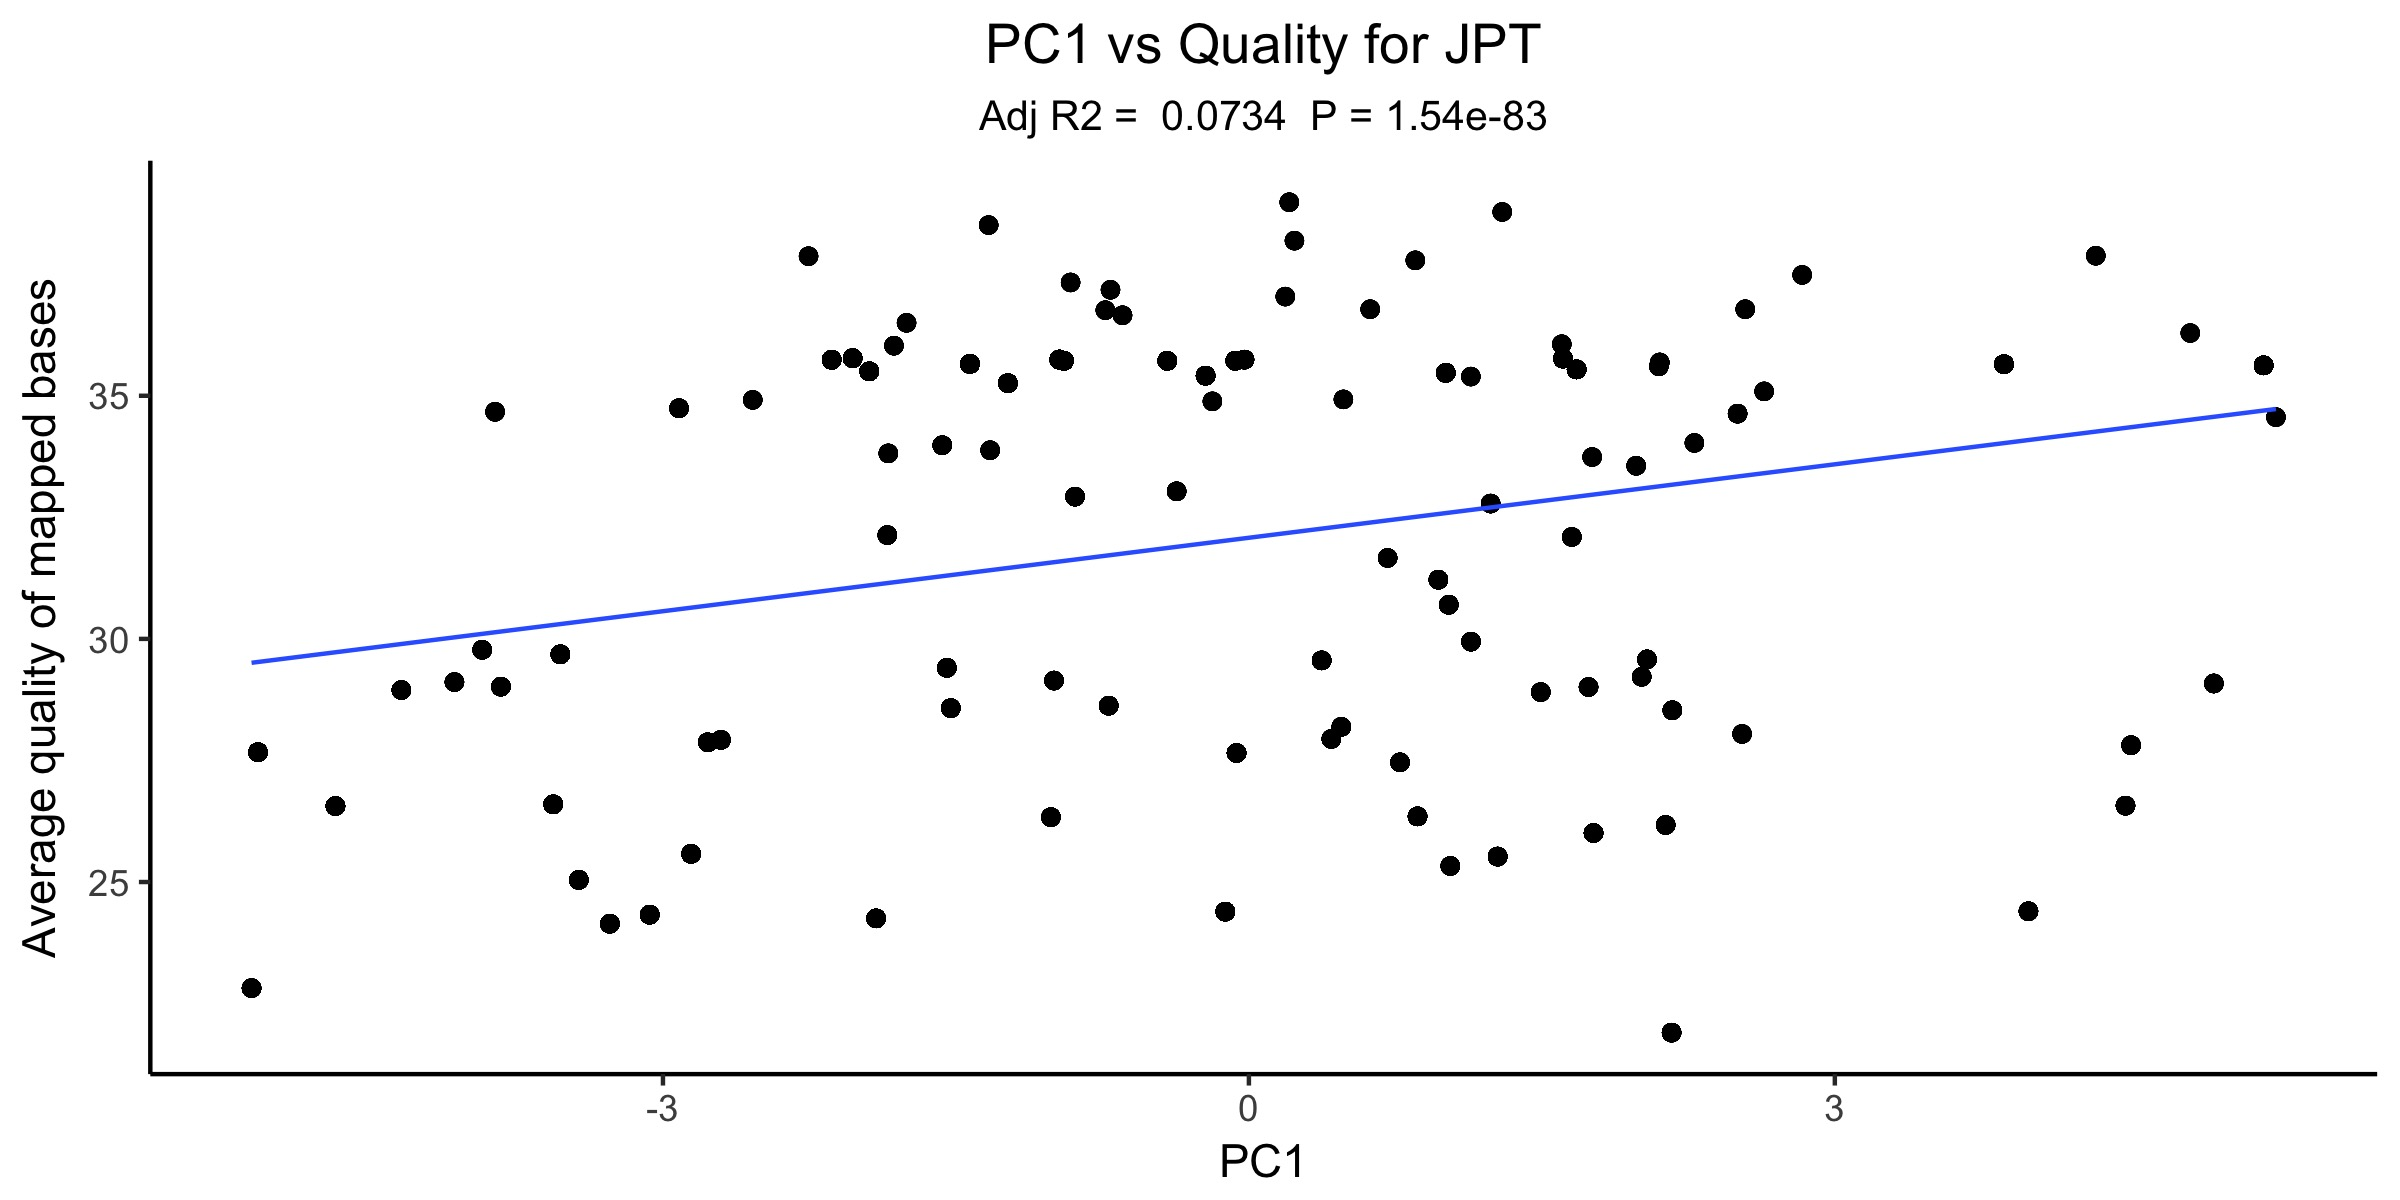
\includegraphics[width=\hsize,keepaspectratio]{PC1_Correlation.jpg}
\caption{Regressions against mean quality per mapped base pair per individual is an excellent correlate with prevalence of the  *AC${\rightarrow}$*CC mutational signature in 1kGP, with individuals with low-quality data showing elevated rates of the signature.  }
\label{PC1_Correlation}
\end{figure}

\begin{figure}
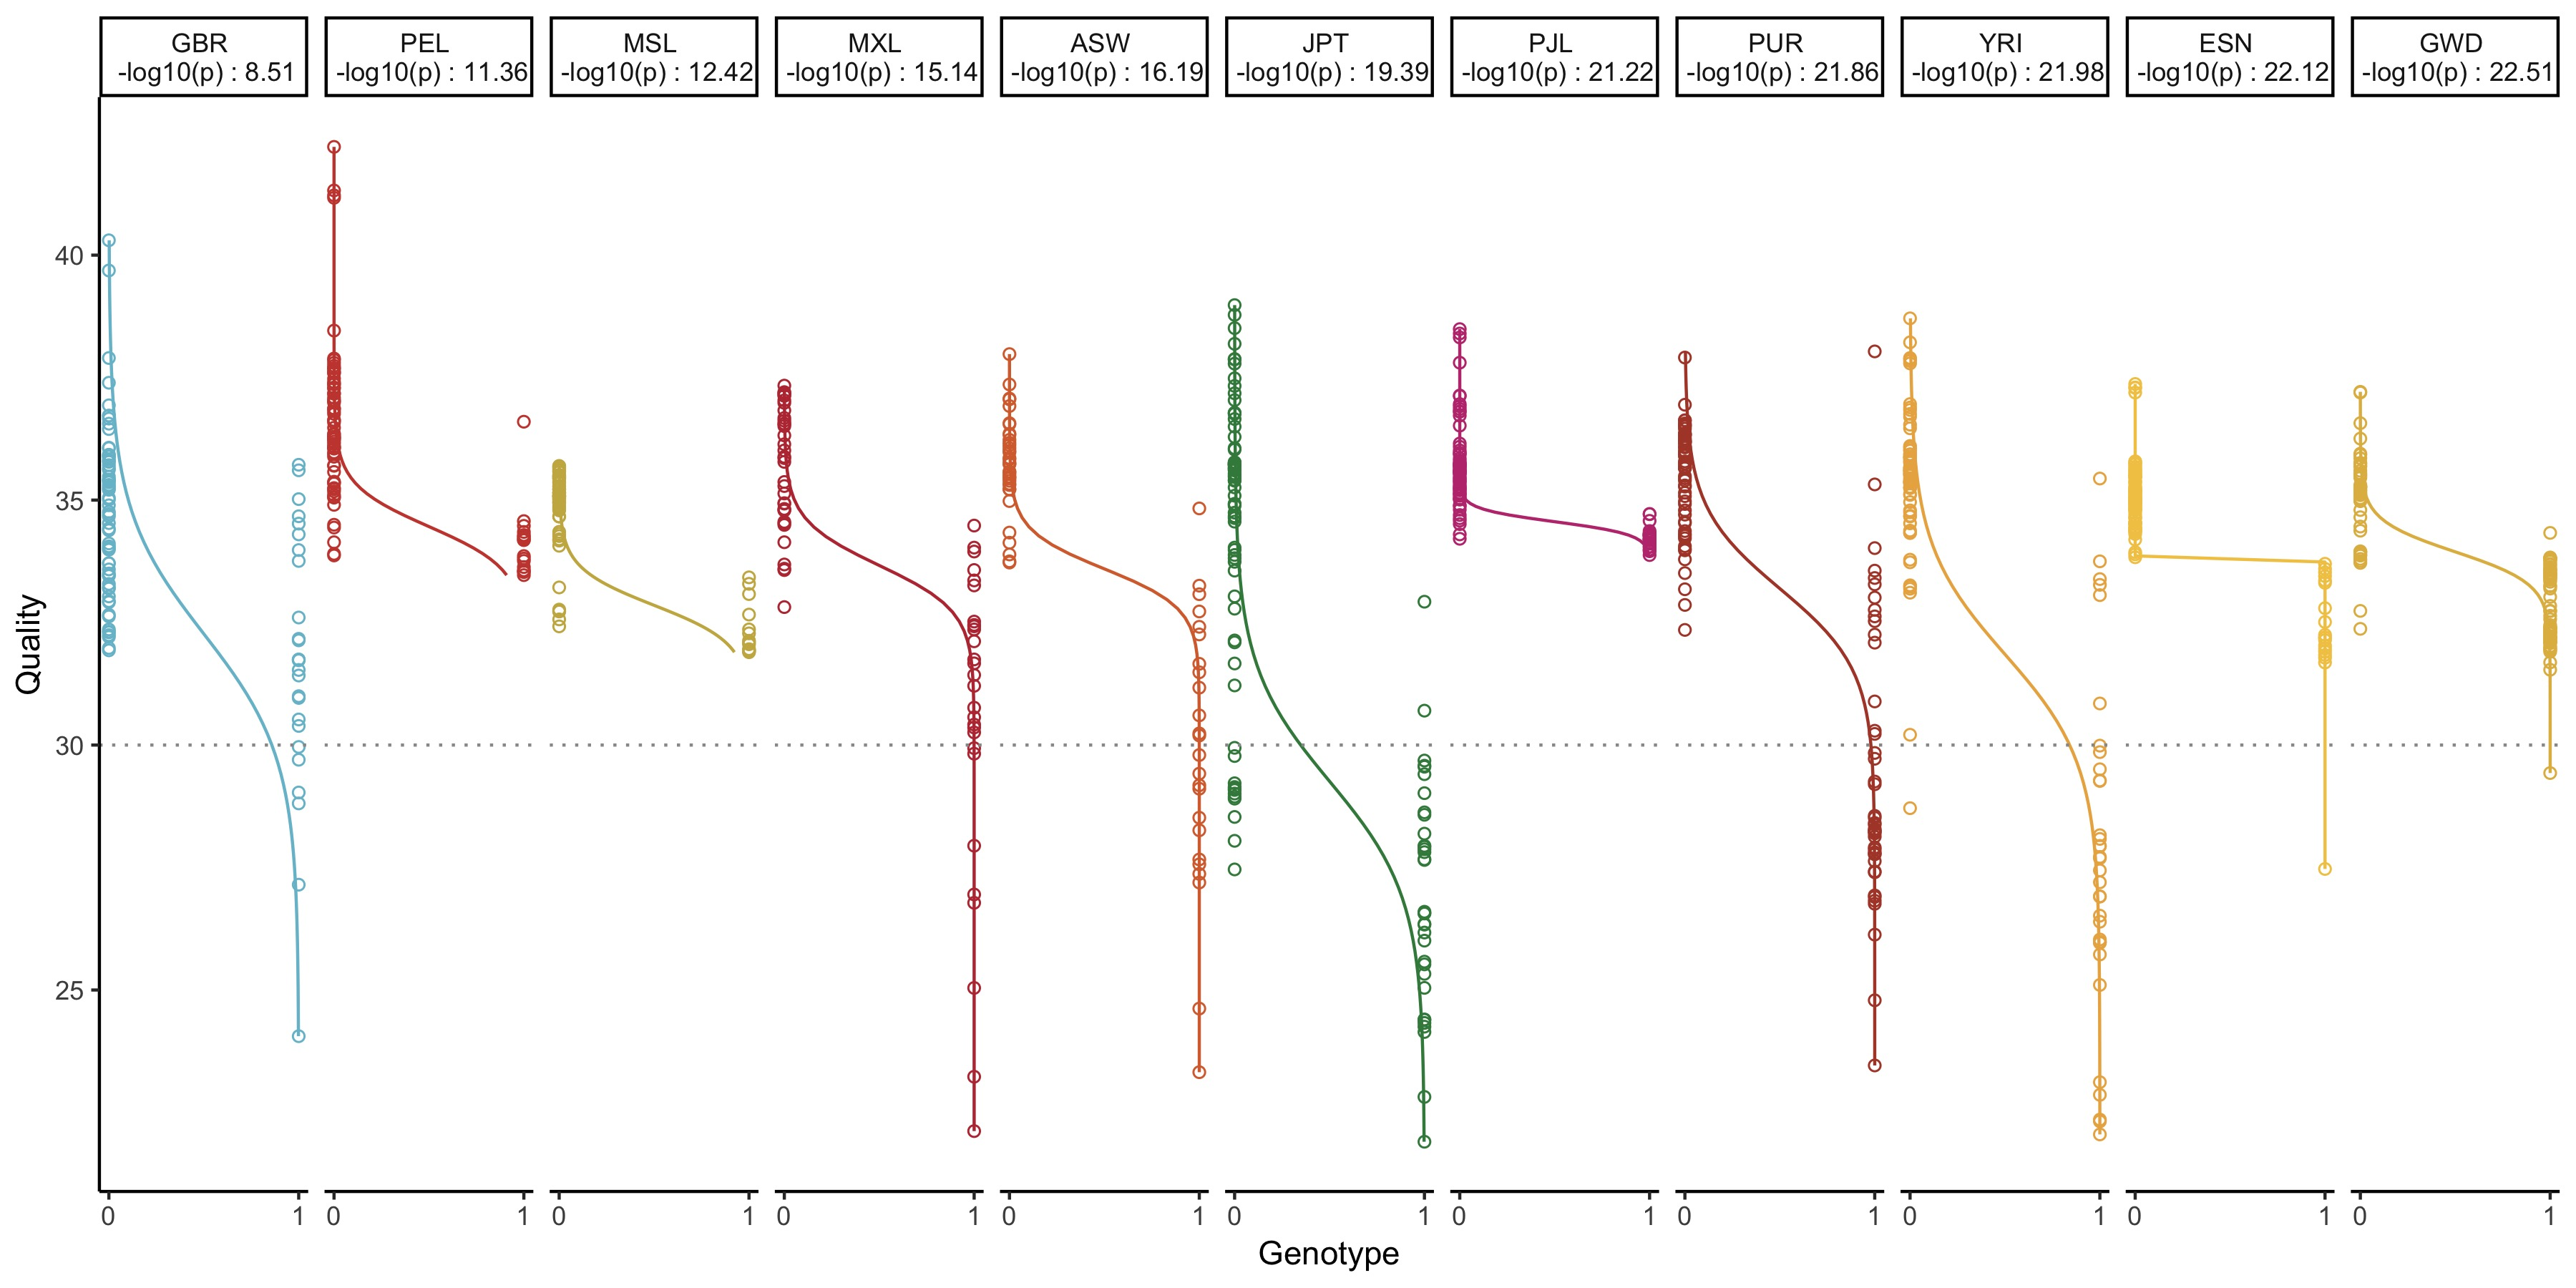
\includegraphics[width=\hsize,keepaspectratio]{RegressionPlot_mostSig2.jpg}
\caption{Logistic regression of the most significantly associated SNP rs75254682 for the populations with significant association to quality.}
\label{MostSig}
\end{figure}

\begin{figure}
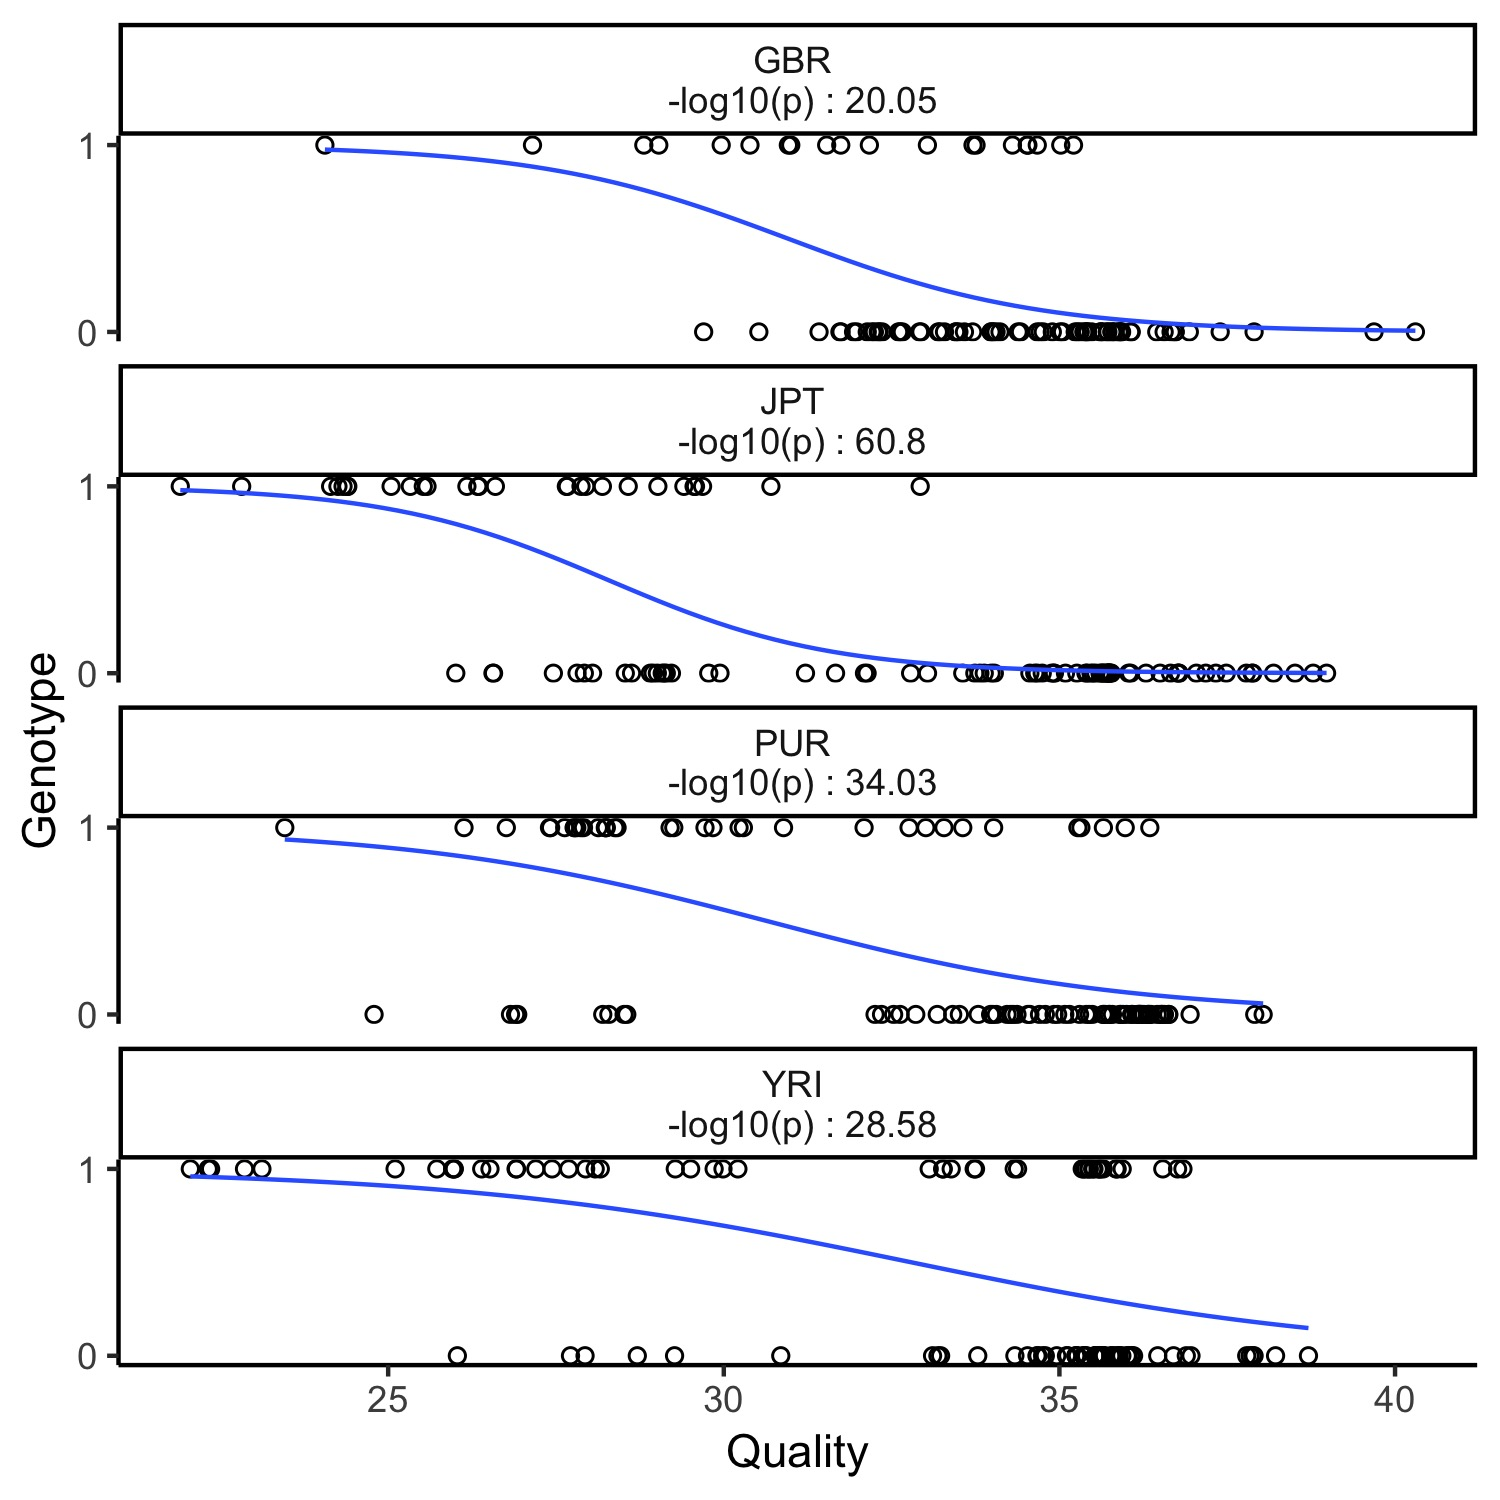
\includegraphics[width=\hsize,keepaspectratio]{RegressionPlot.jpg}
\caption{Logistic regression of rs6057648 for the populations with significant association to quality.}
\label{TwinsSNP}
\end{figure}

\bibliographystyle{plain}
\bibliography{Legacy.bib}

\end{document}
			